\documentclass{beamer}

\usepackage[utf8]{inputenc}
\usepackage{default}
\usepackage{graphicx}


\title{Ol3-Cesium: 3D for OpenLayers}
\subtitle{An exciting library for bringing 3D to your maps}
\author{Guillaume Beraudo}
\institute{Opensource Engineer\\Camptocamp, Switzerland}
\date{FOSDEM Geospatial 2015, February 1\textsuperscript{st}}
\subject{Computer Science}

\hypersetup{colorlinks,urlcolor=blue}
\setbeamertemplate{footline}[text line]{%
  \parbox{\linewidth}{\vspace*{-8pt}OL3-Cesium\hfill\insertshortauthor, Camptocamp}}
\setbeamertemplate{navigation symbols}{}

\begin{document}

  \begin{frame}
    \titlepage
  \end{frame}


  \begin{frame}
    \frametitle{Ol3-Cesium library}

    \begin{center}
      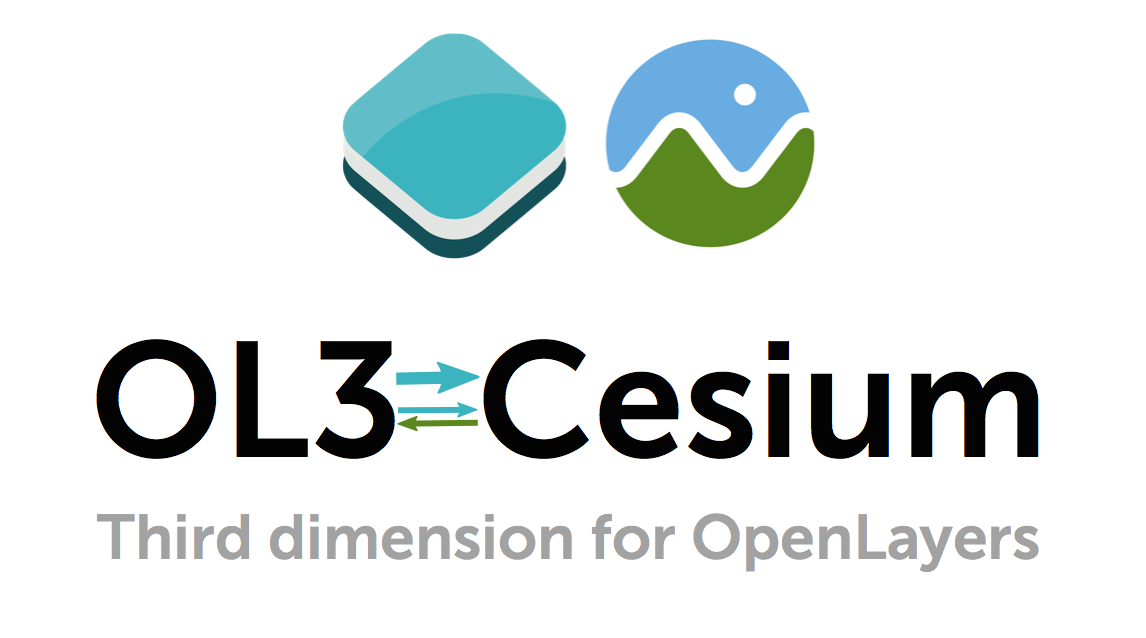
\includegraphics[width=.4\linewidth]{./ol3-cesium-wide_arrows.png}
      % ol3-cesium-wide_arrows.png: 1146x638 pixel, 72dpi, 40.43x22.51 cm, bb=0 0 1146 638
    \end{center}

    \begin{itemize}
     \item Easy setup
     \begin{itemize}
      \item Stacked: \small{\scalebox{.9}[1.0]{\texttt{new olcs.OLCesium(\{map: map\})}}}
      \item Side-by-side: \small{\scalebox{.9}[1.0]{\texttt{new olcs.OLCesium(\{map: map, target: id\})}}}
     \end{itemize}
      \pause
     \item Synchronizers 
      \begin{itemize}
      \item All automatic by default
      \item May be overriden by application
     \end{itemize}
    \end{itemize}
  \end{frame}


  \begin{frame}
    \frametitle{Synchronizations}
    \begin{figure}
    \begin{center}
      \href{http://openlayers.org/ol3-cesium/examples/vectors.html}{
      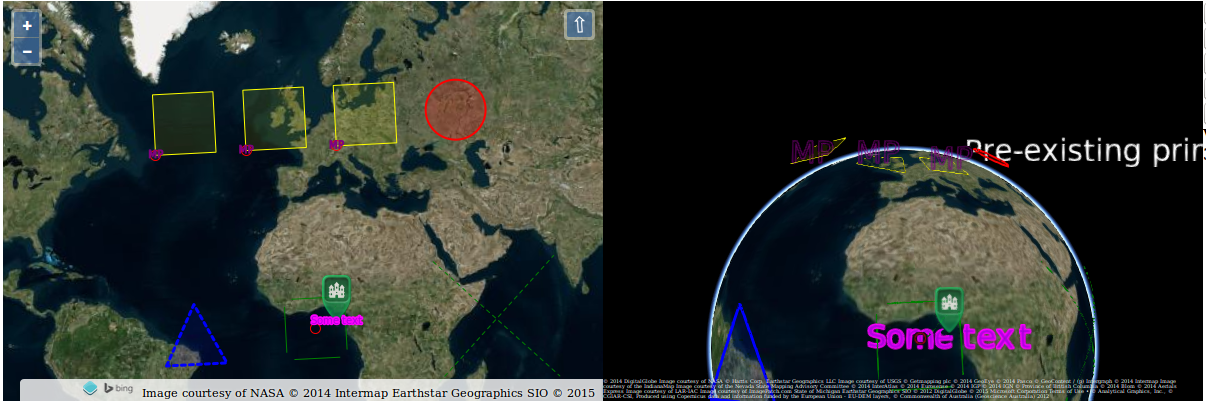
\includegraphics[width=\linewidth]{./capture_vectors_example.png}}
	% capture_vectors_example.png: 1206x406 pixel, 72dpi, 42.54x14.32 cm, bb=0 0 1206 406
    \end{center}
    \href{http://openlayers.org/ol3-cesium/examples/vectors.html}{ol3-cesium/examples/vectors.html}
    \end{figure}

    \begin{itemize}
     \item Ol3 $\rightarrow$ Cesium: unidirectional for layers
     \pause
     \item Ol3 $\leftrightarrow$ Cesium: bidirectional for extent, resolution, rotation
    \end{itemize}
  \end{frame}

  
  \begin{frame}
    \frametitle{Unified 2D/3D interactions}
    \begin{figure}
    \begin{center}
    \href{https://penta.fosdem.org/event/attachment/2871/61}{
      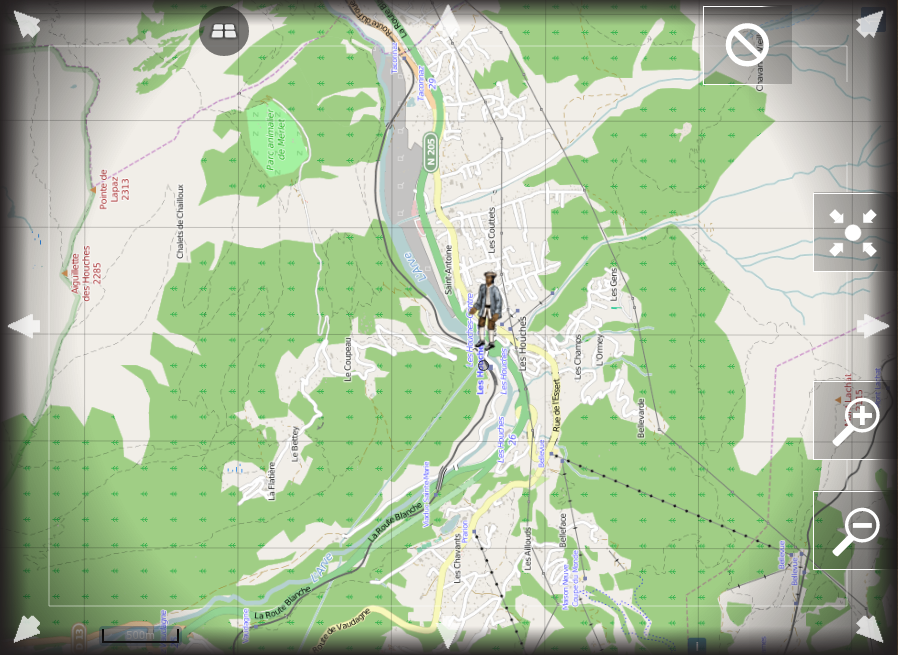
\includegraphics[width=.33\linewidth]{./video1.png}
      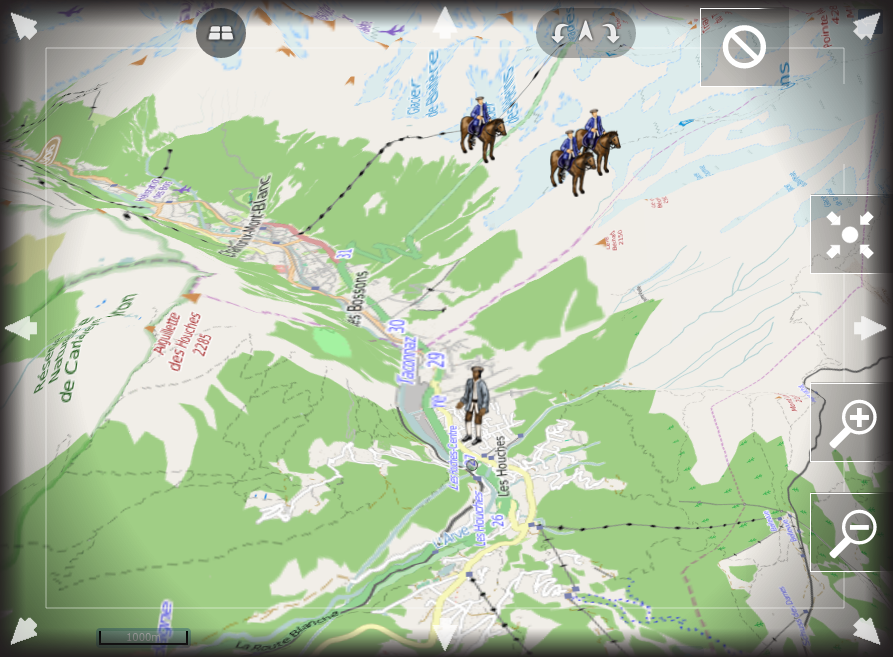
\includegraphics[width=.33\linewidth]{./video2.png}
      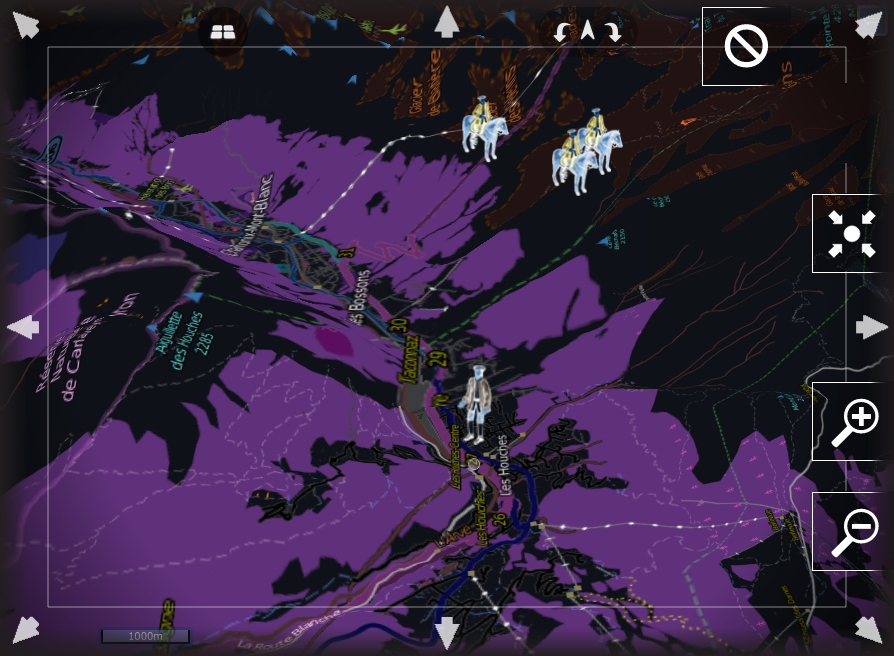
\includegraphics[width=.33\linewidth]{./video3.png}
     }
    \end{center}
    \href{https://penta.fosdem.org/event/attachment/2871/61}{video}
    \end{figure}

    \pause
    \begin{itemize}
     \item Shared 2D and 3D views, controls, POI   edition
     \item Interactions spanning between 2D and 3D
    \end{itemize}
  \end{frame}

  
  \begin{frame}
    \frametitle{Community}
    \vspace{-20pt}\begin{center}
      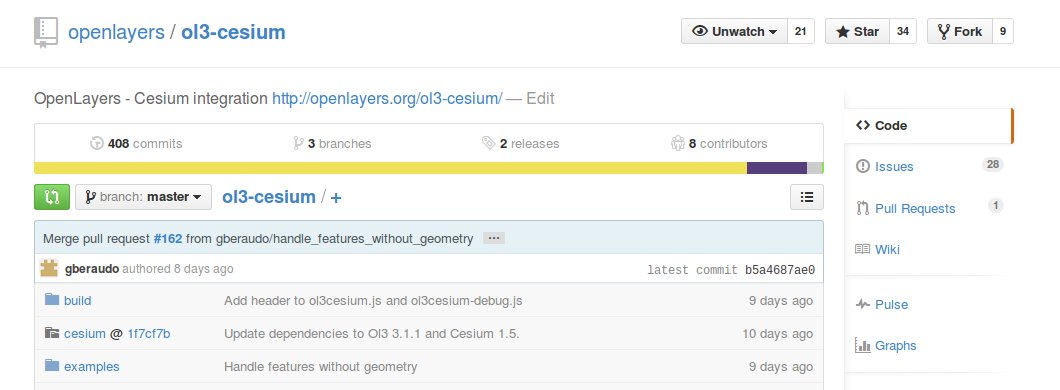
\includegraphics[width=0.9\linewidth]{./github2.png}
    \end{center}
    
    \begin{itemize}
     \item Started by three companies, 408 commits, 8 contributors
     \pause
     \item Monthly releases, check \href{https://github.com/openlayers/ol3-cesium/blob/master/CHANGES.md}{CHANGES.md}
     \pause
     \item Young project where you can have a big impact
     \begin{itemize}
       \item Feedback
       \item Issues
       \item Contributions
     \end{itemize}
    \end{itemize}
  \end{frame}


  \begin{frame}
    \frametitle{Future}
    \begin{itemize}
      \item Continue improving policies and code
      \item Add more functionalities (features on terrain, night mode, \dots)
      \item Keep up with Ol3 and Cesium pace
      \item Allow even more customizations
      \item \dots
    \end{itemize}
  \end{frame}

\end{document}
